\documentclass[a4paper]{article}

%% Language and font encodings
\usepackage[english]{babel}
\usepackage[utf8x]{inputenc}
\usepackage[T1]{fontenc}
\usepackage{graphicx}
\usepackage{caption}
\usepackage{subcaption}
\usepackage{eurosym}
\usepackage{multirow}
\usepackage{footnote}
\usepackage{listings}
\usepackage{color}
\usepackage{pdfpages}

%% Sets page size and margins
\usepackage[a4paper,top=3cm,bottom=2cm,left=3cm,right=3cm,marginparwidth=1.75cm]{geometry}

%% Useful packages
\usepackage{amsmath}
\usepackage{graphicx}
\usepackage[colorinlistoftodos]{todonotes}
\usepackage[colorlinks=true, allcolors=blue]{hyperref}
\begin{document}

\begin{titlepage}

\newcommand{\HRule}{\rule{\linewidth}{0.5mm}} % Defines a new command for the horizontal lines, change thickness here

\center % Center everything on the page
 
%----------------------------------------------------------------------------------------
%	HEADING SECTIONS
%----------------------------------------------------------------------------------------

\textsc{\LARGE Ecole Polytechnique de Bruxelles}\\[1.5cm] % Name of your university/college
\textsc{\LARGE University of Leeds}\\[1.5cm]
\textsc{\large Johnston Lab Internship}\\[0.5cm] % Minor heading such as course title

%----------------------------------------------------------------------------------------
%	TITLE SECTION
%----------------------------------------------------------------------------------------

\HRule \\[0.4cm]
{ \huge \bfseries Technical description and User guide: Motion Sensor for behavioral rodent experiments using optical computer mice}\\[0.4cm] % Title of your document
\HRule \\[1.5cm]
 
%----------------------------------------------------------------------------------------
%	AUTHOR SECTION
%----------------------------------------------------------------------------------------

\begin{minipage}{0.4\textwidth}
\begin{flushleft} \large
\emph{Author:}\\
Maxime \textsc{Verstraeten} % Your name
\end{flushleft}
\end{minipage}
~
\begin{minipage}{0.4\textwidth}
\begin{flushright} \large
\emph{Supervisor:} \\
Jamie \textsc{Johnston}\\[0.3cm] % Supervisor's Name
\end{flushright}
\end{minipage}\\[2cm]

% If you don't want a supervisor, uncomment the two lines below and remove the section above
%\Large \emph{Author:}\\
%John \textsc{Smith}\\[3cm] % Your name

%----------------------------------------------------------------------------------------
%	DATE SECTION
%----------------------------------------------------------------------------------------

{\large \today}\\[2cm] % Date, change the \today to a set date if you want to be precise

%----------------------------------------------------------------------------------------

\vfill % Fill the rest of the page with whitespace

\end{titlepage}


\noindent\rule{\textwidth}{1pt}

\tableofcontents

\newpage

\listoffigures

\newpage



\section{Introduction}
This user guide intends to provide the user with the information required to use and understand the ball motion sensor device developed at JohnstonLab as well as giving some clues regarding troubleshooting and help with the other tools developed as well.\\

This device was developed as part of my internship at JohnstonLab (Leeds University, UK) during my master's years as a student engineer from the Université Libre de Bruxelles, Belgium.

This device is part of the rig that allows the lab to perform in-vivo measurements and experiments on mice. This device gathers data from optical computer mice to use them as motion sensor for behavioral studies on mice.\\

Note: The workflow, thoughts, issues, ... for this project are discussed in my OneNote.\\

The latest software and documentation updates are available on my Github: \url{https://github.com/maverstr/PS2-Motion-Sensor}

\section{Objective}
When performing behavioral studies on mice, it is interesting to be able to set up a Virtual Reality setup. To do so, the mouse should be able to move freely but still be under the field of view of the microscope, like on a treadmill. The best 3D treadmill is obviously a sphere. 
This is why for that kind of experiment, the mouse will be running on a Styrofoam ball, held above a bowl by air pressure (this allows minimal resistance between the ball and the bowl).
Now to be able to perform virtual reality experimentation, one must know how the mouse, or at least how the ball, moves.

Such device exist on the market but with a very high price.

\begin{figure}[h!]
    \centering
    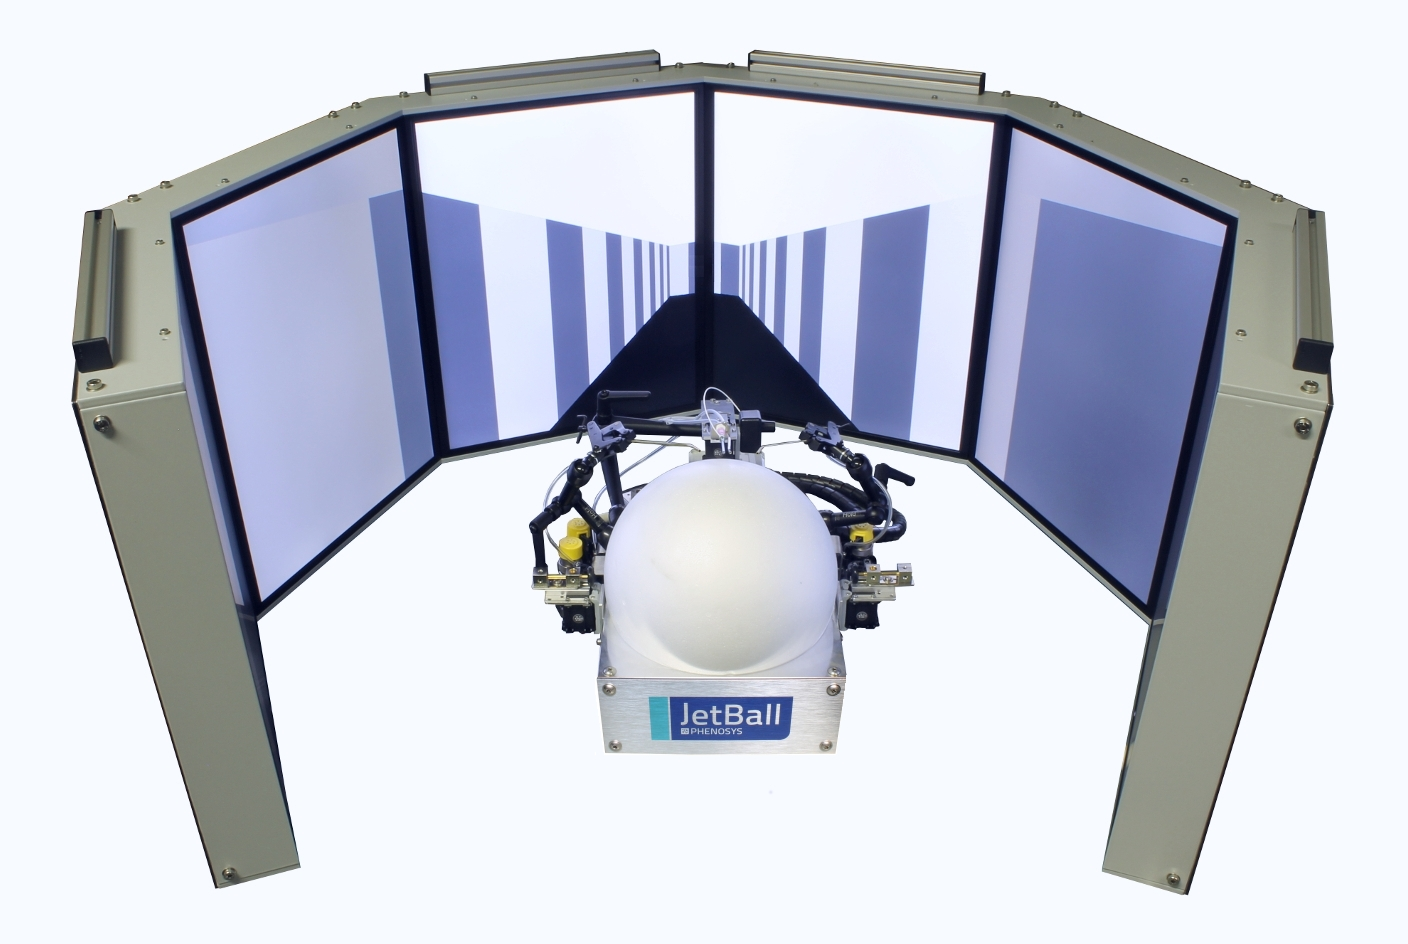
\includegraphics[width = 10cm]{images/VR.jpg}
    \caption{Market VR setup}
    \label{fig:vr}
\end{figure}


The goal of this device is therefore to act as a motion sensor for VR experimentation, with a very inexpensive setup.

\section{Hardware}
The device is extremely simple and is composed of mainly 4 parts:
\subsection{Optical mouse}
The main element is an optical computer mouse that will act as the sensor.
Computer mice have a high sampling rate for computing the deltaX and deltaY and are capable of a great precision.
The main characteristic is the dpi (dot per inch) as it will limit the maximum speed of movement detection and the accuracy. 
We use a Perixx PERIMICE-201 II (800 dpi and around 7£).

The optical mice can be taken apart to use only the PCB and the lens that come with it, but it requires to do so meticulously. By designing a mouse holder in CAD and keeping the PS/2 connector, it becomes basically "plug\&play" and allows easy replacement.

\begin{figure}[h!]
    \centering
    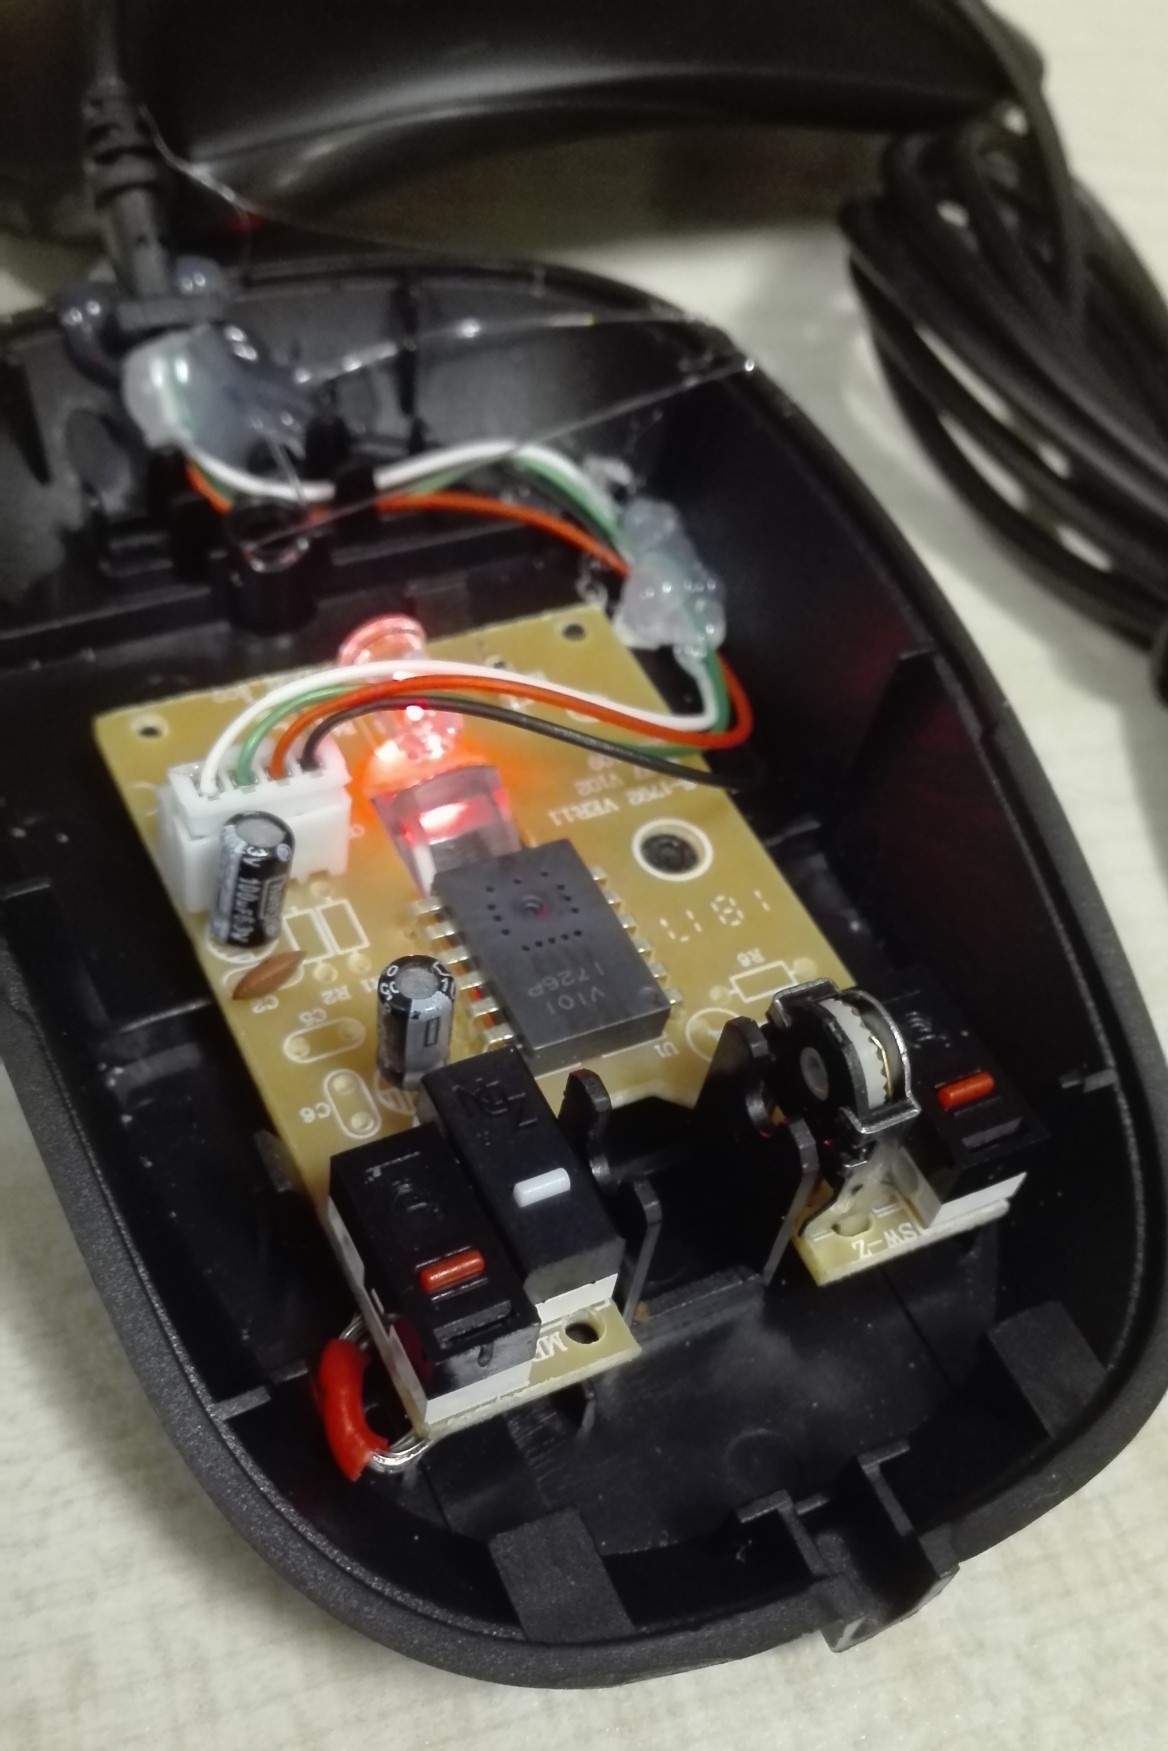
\includegraphics[width = 8cm]{images/mouse.jpg}
    \caption{Disassembled mouse}
    \label{fig:mouse}
\end{figure}

\subsection{PS/2 connector}
The mice used in everyday life are either USB or PS/2.
We want to use the PS/2 connectors as they are easier to "hack" and get data from them.

\begin{figure}[h!]
    \centering
    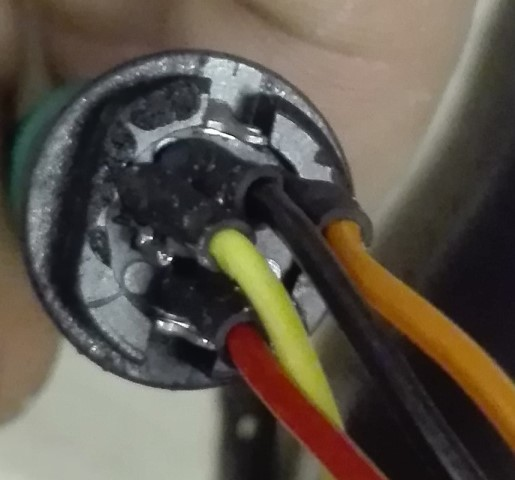
\includegraphics[width = 5cm]{images/ps2.jpg}
    \caption{PS2 Connector}
    \label{fig:connector}
\end{figure}


These connectors features ground (pin3), 5V(pin 4), SDA (pin 1) and SCL (pin 5).
Note that it is reversed for male connectors of course.

\begin{figure}[h!]
    \centering
    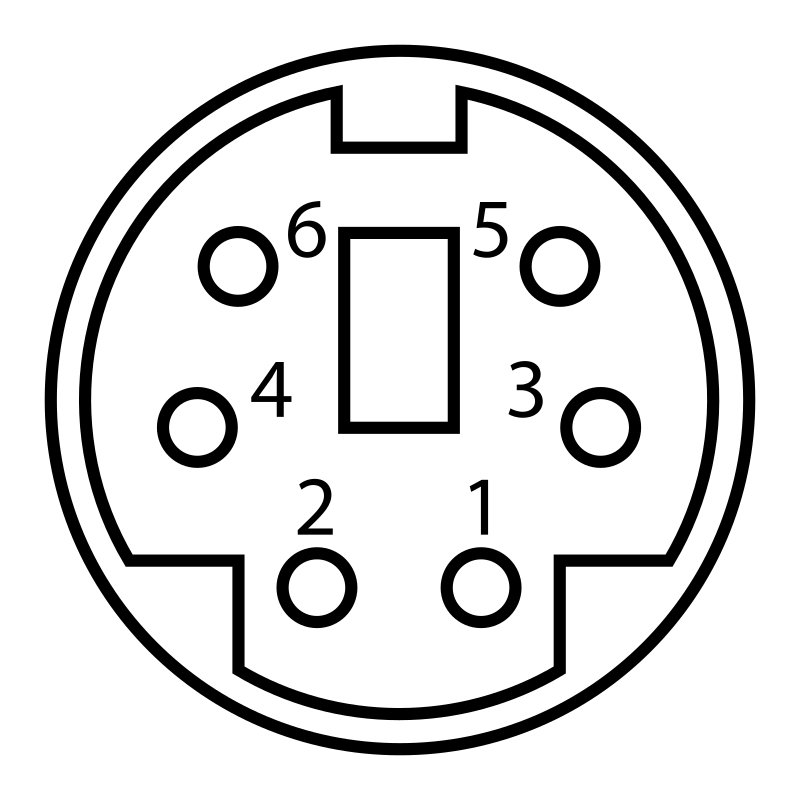
\includegraphics[width = 5cm]{images/PS2.png}
    \caption{PS2 connector scheme (wikipedia)}
    \label{fig:PS2}
\end{figure}



\subsection{Mouse holder}
To hold the mice in place very close to the ball, I designed 3D-printed holders.

\begin{figure}[h!]
    \centering
    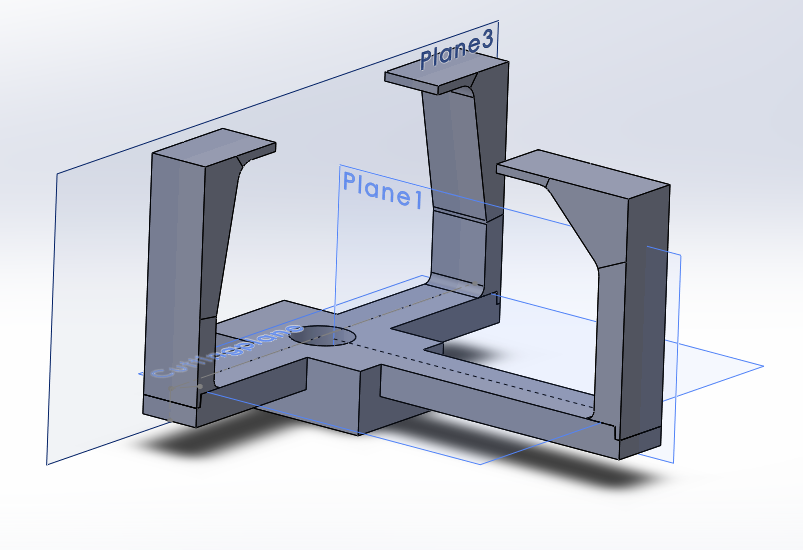
\includegraphics[width = 8cm]{images/cad1.png}
    \caption{mouse holder CAD design}
    \label{fig:cad1}
\end{figure}

\begin{figure}[h!]
    \centering
    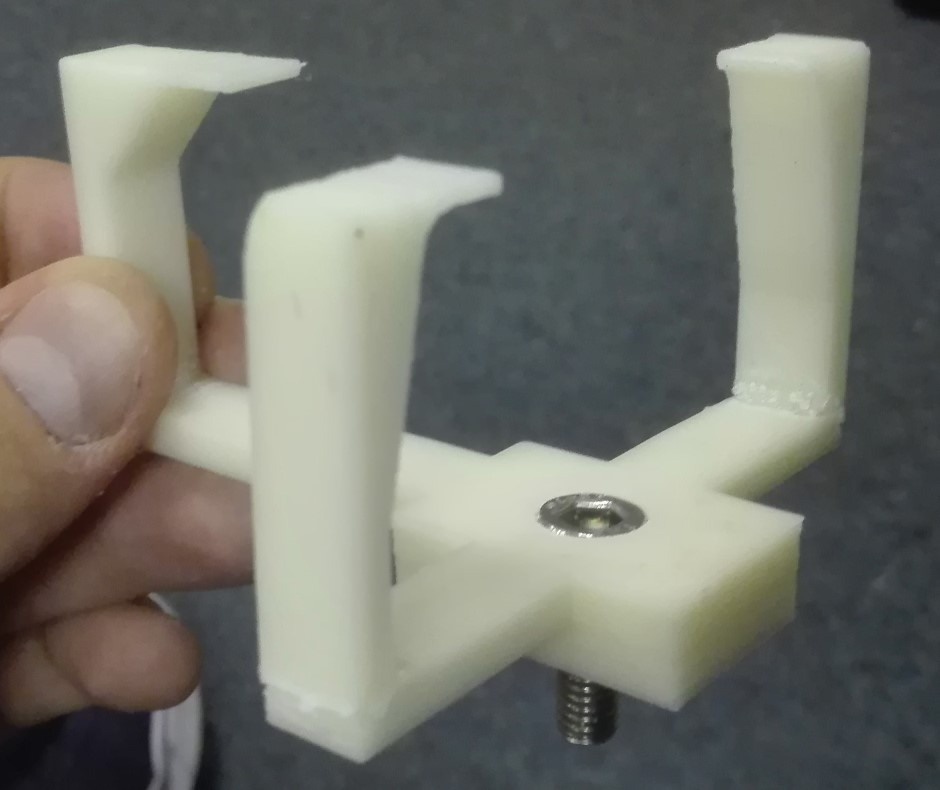
\includegraphics[width = 8cm]{images/cad2.jpg}
    \caption{Printed mouse holder}
    \label{fig:cad2}
\end{figure}

\begin{figure}[h!]
    \centering
    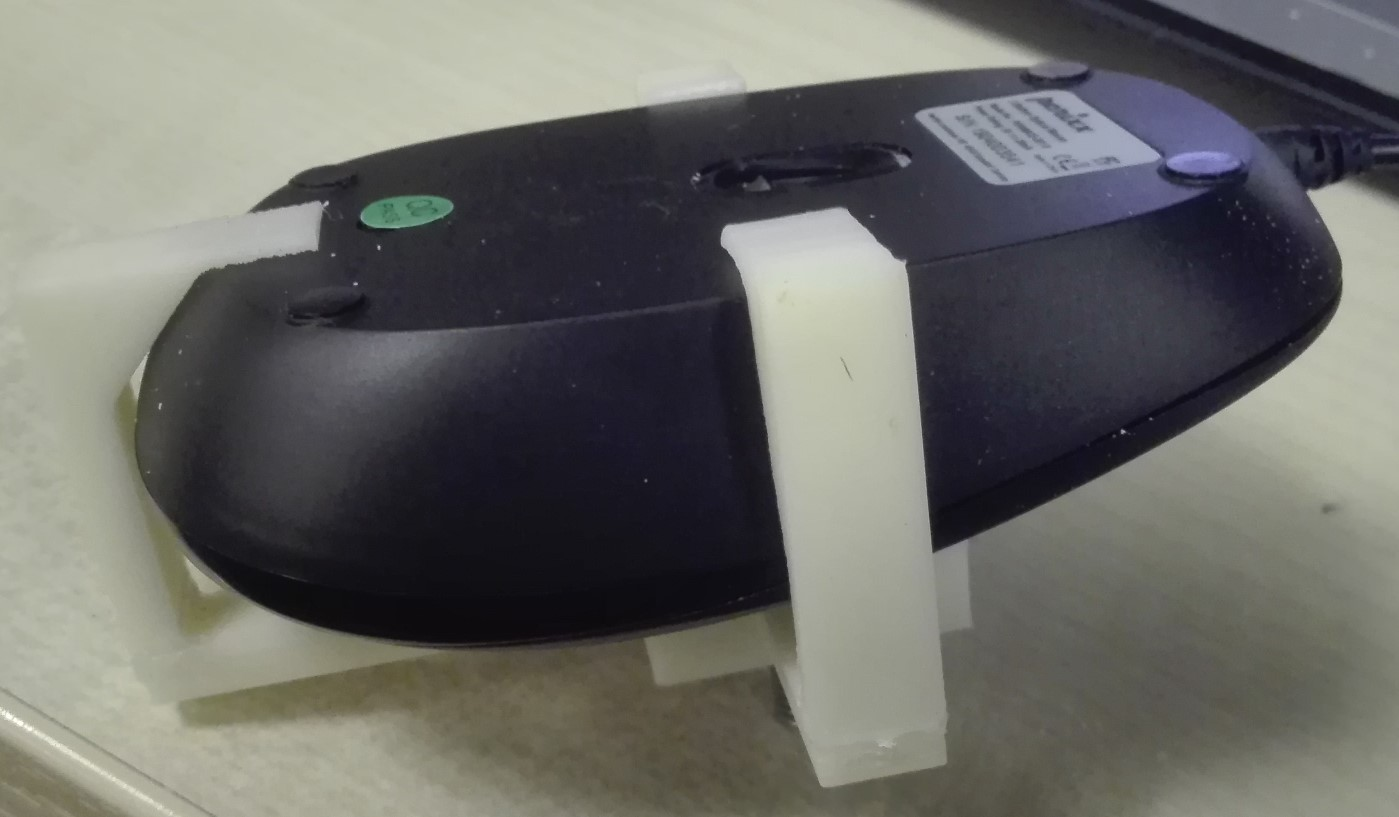
\includegraphics[width = 8cm]{images/cad3.jpg}
    \caption{Mouse held}
    \label{fig:cad3}
\end{figure}

The mouse holders can be attached to the microscopic rig through the bolt going through it.

\subsection{Microcontroller}
The logic part of the device is handled by an Arduino Mega (even though any Arduino or other µC will do as long as it has 4 digital inputs, 5V supply and a connection to ground). It provides Ground and 5V supply and receives SDA and SCL for each mouse.
Note that even though PS/2 is using SDA and SCL, the µC does not require I2C ports with the used libraries. Any digital inputs will do.

\section{Software}
A PS2 library is able to get the deltaX and deltaY every frame. I simply print the correct values to the Serial and perform vector computation in polar coordinates.

The data can also be transferred over I2C to another µC if needed(but it is not the case in our device plan).

\section{How to use?}
Simply plug the mice into the hacked PS2 connectors and plug the Arduino. It will immediately start sending the data over Serial.

This data can also easily be transferred over I2C.

\begin{figure}[h!b!t!]
    \centering
    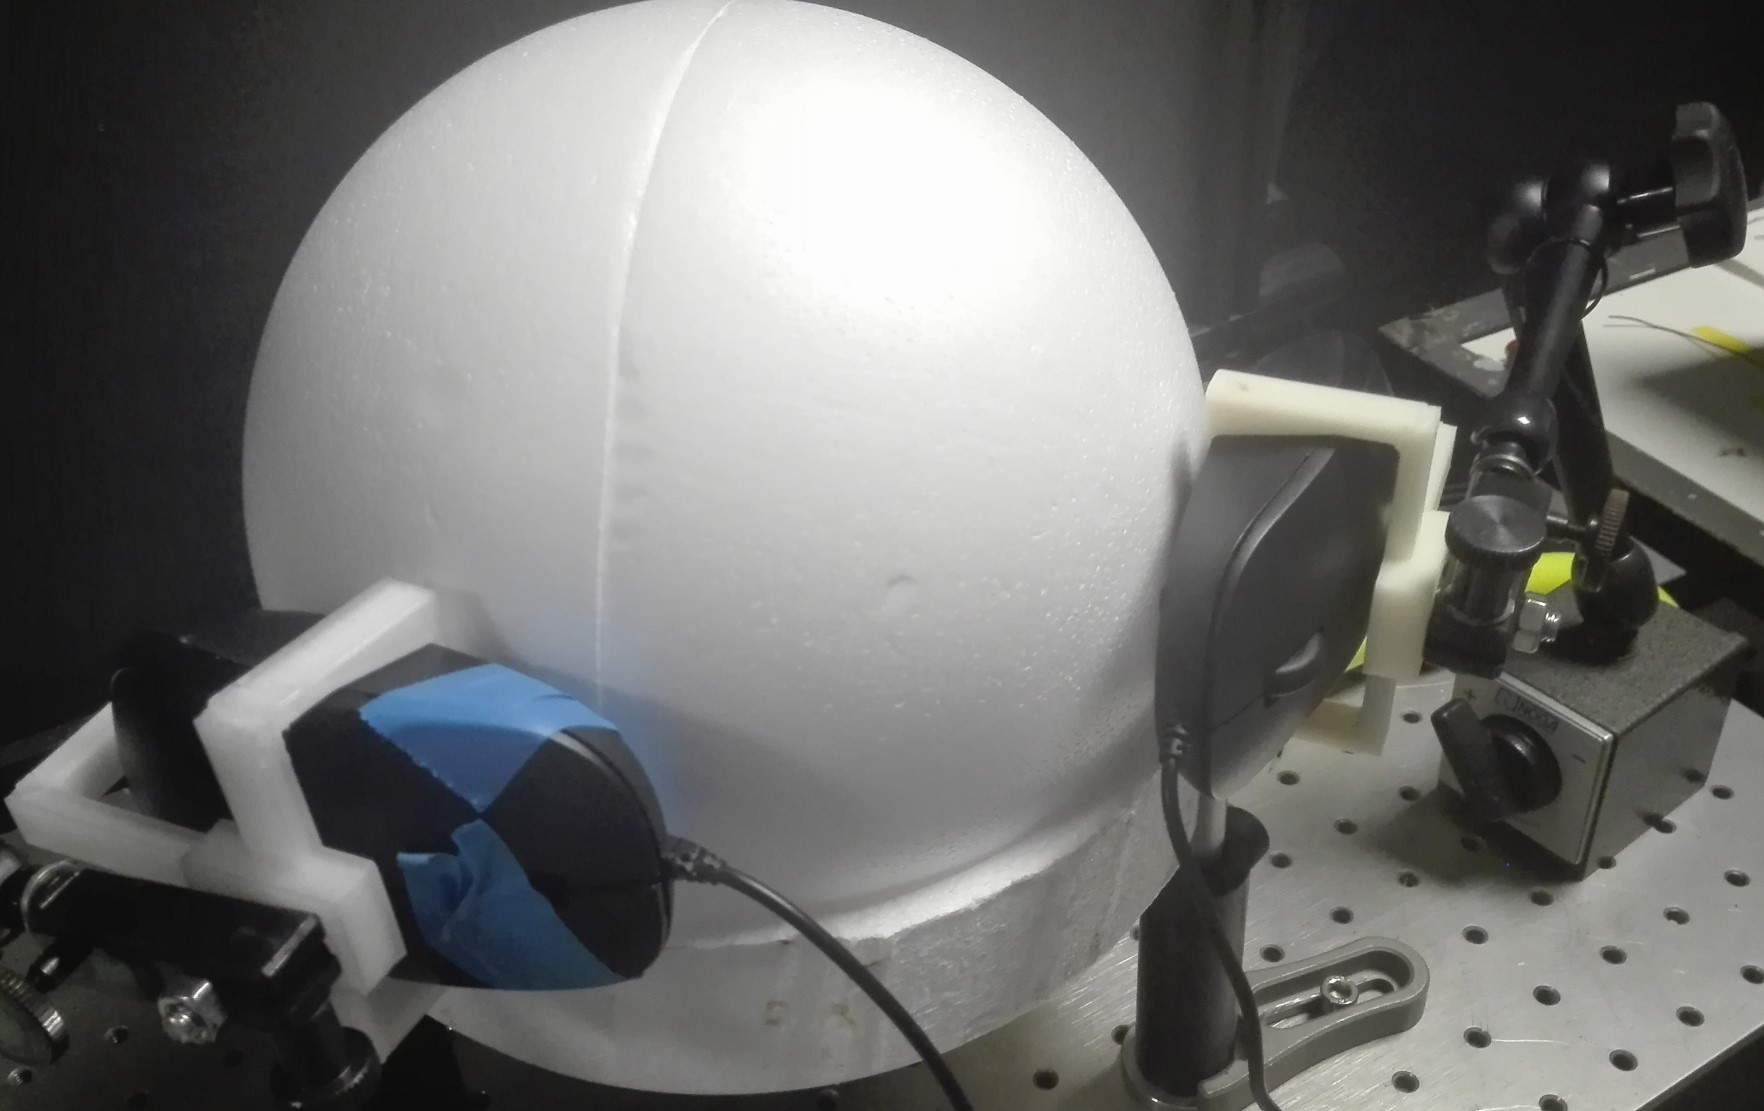
\includegraphics[width = 10cm]{images/setup.jpg}
    \caption{Sensor setup}
    \label{fig:setup}
\end{figure}

\section{Expected Results}
The Arduino should send the motion over Serial. This can be checked through the Arduino IDE. Moreover, the Processing3 script (section \ref{processing}) will draw the corresponding motion on a map (Figure \ref{fig:procMap}).



\subsection{From mice data to movement mapping}
The libraries used allow to get the X and Y data for each mouse as an 8-bit signed value (-127 to +127). Given that the mice are placed 90 degrees apart from each other on the side of the ball (the rodent running on top), a mouse can detects the X movement of the ball (i.e. rotation left/right from a top view of the rodent, perfect crab-walk), the other can detect the Y (i.e. the rodent running forward/backward) and both of them also detect the Z axis movement (i.e. the rodent is turning). 

The redundancy of Z can be either discarded on one mouse or used for data verification.

The conversion to an actual map of motion is done by using a rotation matrix using Z as the rotation angle.
It is obviously necessary to calibrate the axis (i.e. how many dots for one single 360 degrees rotation. In our case, 13 000 is a good approximation).


We can then decide to either output the absolute values on the Serial and/or to the I2C bus to the microscopic rig and ScanImage or make the computation to output the values with the rotation around the Z axis.

\begin{figure}[h!]
    \centering
    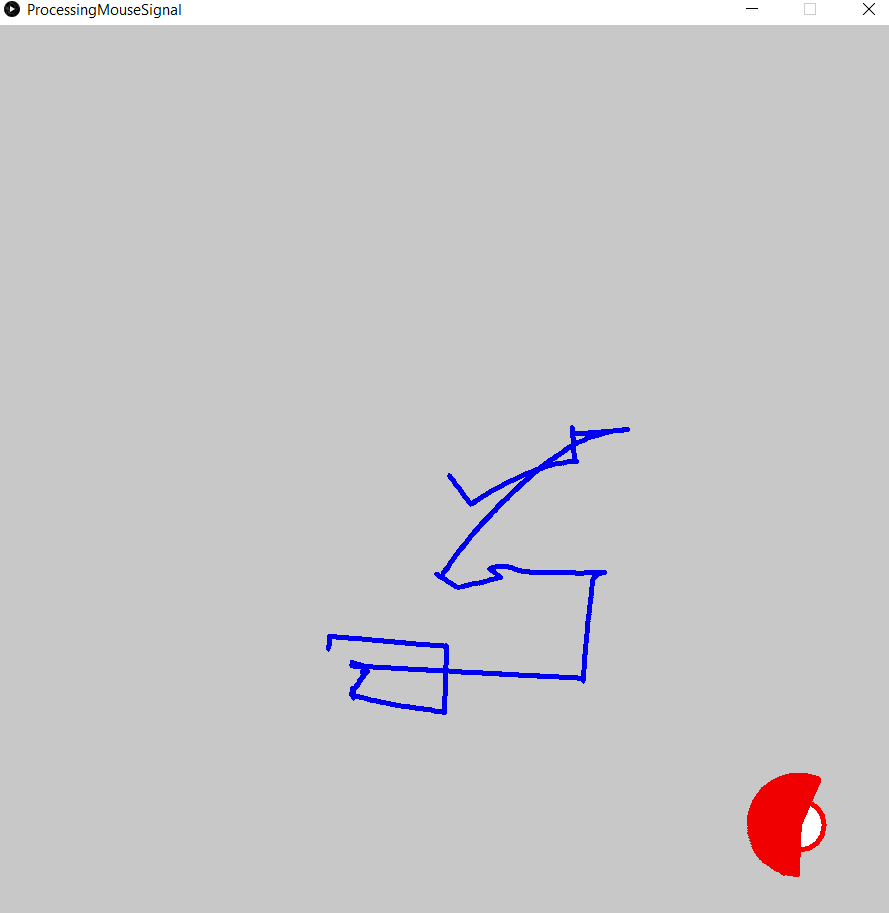
\includegraphics[width = 8cm]{images/processingMap.PNG}
    \caption{Map drawn on Processing3}
    \label{fig:procMap}
\end{figure}

\section{Troubleshooting}
\subsection{The motion map does not correspond to actual movements}
One mouse handles X and Y movement, the other will handle Z and (redundant) Y. It is therefore important to place them 90 degrees apart from each other as well as perpendicular to the ball.
\section{Improvements}
\subsection{laser mouse}
The mouse used for the moment is an optical mouse, which uses a LED as light source which is cheap. The mouse could be replaced by a laser mouse which uses a laser as the source.
In both cases, a CMOS is used as the sensor to detect the variation of the surface under the mouse and compute the movement.

Laser mice usually have higher DPI, which means they can track more "dots per inch" and therefore are more sensitive.

Moreover, the optical mice only sense the top of the surface while the laser goes more deeply and see smaller peaks and valleys in the surface. This leads to more jittery data at low speed but a laser mouse is able to work on any surface, even glossy ones (which is somewhat the case with the Styrofoam ball).

\subsection{higher DPI}
Having a higher DPI is useful to be more sensitive and allow fast movements to be recognized correctly. Indeed, the PS/2 connector will only output 8-bit signed values. So it cannot send more that -127 to +127 every sampling rate (which depends on the mouse and the Arduino code; in early testing the sampling rate was about 60Hz). 
Having a higher DPI means that the max speed will be reduced as the maximum 8-bit values will be reached on a smaller distance (more dots per inch) but the mouse will be more sensitive.
All in all, a higher DPI means a more sensitive mouse, but one must be careful not to decrease the max speed too much otherwise the data will be saturated all the time.

\subsection{Direct use of the sensor}
USB mice are already largely prefered over PS/2 mice and it might get difficult in the coming years to find working PS/2 mice. Moreover, the CAD holder is designed for a specific mouse model.
It might be interesting to directly wire the connectors to the PCB (easily done thanks to the MTA connectors) and disassemble the mouse or even directly use the sensor.
This however requires more work in case of replacement and it might get too technical for a biology lab for such a small improvement. The "plug\&play" approach proposed here is therefore preferred.

\section{Other tools}
\subsection{Processing3 Visualisation}
\label{processing}
I developed a Processing3 (Java) script that gathers data from the Serial port and draws the motion map corresponding to the mouse movement. This allows easy debugging and understanding of how the device works.

To use it, simply plug the Arduino into the computer and select the correct COM port in Processing. A gray window opens, press any key to start and move the mice to observe the drawing.

The device can be seen on video: \url{https://youtu.be/RcX8a1zjNxQ}

\appendix


\bibliographystyle{alpha}
\bibliography{biblio}

\end{document}